In the following test experiments we evaluate the benefits of passing additional information through the layers of the hypervisor and guests for profiling.  Unless otherwise noted, each experiment is performed on a \emph{Personal} and \emph{Business} scale virtualization platform (Table \ref{virtSize}).  Both systems have CentOS and Xen Server installed (Table \ref{softStack}) for the software stack installed.

\subsection{External machine interference}
In this experiment, we show the memory and I/O interference from external systems.  
Without any changes in the guest running the benchmark, there is a significant drop in performance when external systems run concurrently.  
However, monitoring resources in only the guest domain provides little information about the performance problems. 

To begin this exercise, we divide the physical memory and CPUs into four equal parts and create four individual guest virtual machines (Dom1 - Dom4).  
Each virtual machine is given 25\% of the available resources so that no guest virtual machine would interfere with another machine if they were on separate physical systems.  
We start only our Dom1 machine and run our experimental test with PGbench.  
On our \emph{Business} Dell server, Dom1 is allocated 2GB vRAM and 2 vCPU, while on our \emph{Personal} IBM server Dom1 is given 512MB vRAM and 1 vCPU.  

\subsubsection{Database Size}
The test starts by initializing a very small database and runs PGBench and collect the TPS.  
Then we increase the DB size slightly and run the benchmark again.  
After repeating this process several times, we can see that when the DB size changes to an I/O bound system its performance drops significantly (Figure \ref{fig:smallIO}).  
This is due to the fact that it must fetch database rows from the disk and it is much slower.  

\begin{figure}[!h]
  \begin{center}
  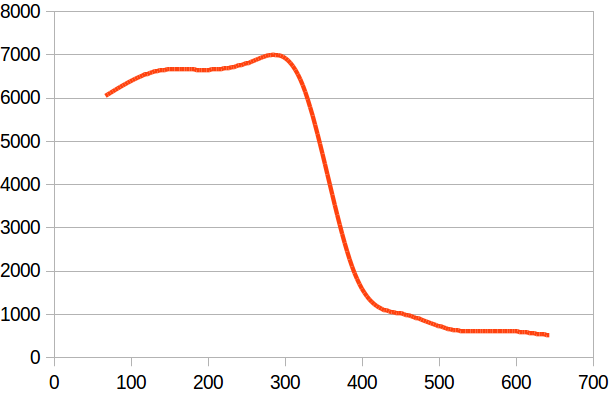
\includegraphics[width=4in]{images/SmallScale.png}
  \caption{TPS on our IBM x3650 system with 1 vCPU and 512KB vRAM. It changes from a memory bound application to an I/O bound application when the DB size approache the available RAM.}
  \label{fig:smallIO}
  \end{center}
\end{figure}

\begin{description}
  \item[Small DB] The working set can fit into main memory.  Performance is based on Memory.
  \item[Medium DB] The working set is swapped to disk occasionally. Performance is moving from Memory to I/O.
  \item[Large DB] Most reads need to go to disk.  Performance is based on Disk I/O.
\end{description}

% Section 7.1.2
\subsubsection{With Interference}
Then we simulate external machine interference by running Dom1 concurrently with Dom2, Dom3, and Dom4. 
Each of the Dom2 - Dom4 systems are configured the same as Dom1.  
We create a 2 GB database on each guest of the Dell, and a 1GB database on each guest of the IBM.  
We run a PGBench in a loop to continuously create I/O interference on each external guest machine (Dom2 - Dom4) while going from a small DB to a large DB on Dom1.

We measure the results of the benchmark on Dom1, while the other 3 guest domains are causing interference.  
When the system is not I/O bound (Small DB) there is about a 28\% drop in performance (4434 TPS - 3208 TPS) on the IBM server and little change in the Dell server (Table \ref{fig:tps1}).  
On both servers the guest becomes an I/O bound system quicker,  and there is significant interference from the I/O on both servers for a large database.

\begin{table}[h]
\begin{subtable}[h]{0.45\textwidth}
  \begin{tabular}{ l | r | r | r }
    DB Size & Single & Interfernce & Drop \\
    \hline
    Small & 4434 & 3208 & 28\% \\ \hline
    Medium & 2149 & 216 & 90\% \\ \hline
    Large & 260 & 197 & 24\% \\  \hline
    \hline
  \end{tabular}
\caption{IBM x3650 with 2GB RAM:  Each Guest domain has 512MB Allocated.}
\end{subtable}
\hfill
\begin{subtable}[h]{0.45\textwidth}
  \begin{tabular}{ l | r | r | r }
    DB Size & Single & Interference & Drop \\
    \hline
    Small & 5772 & 5734 & 0.7\% \\ \hline
    Medium & 1608 & 162 & 90\% \\ \hline
    Large & 359 & 82 & 77\% \\  \hline
    \hline
  \end{tabular}
\caption{Dell T410 with 12GB RAM:  Each Guest domain has 2GB Allocated. }
\end{subtable}
\caption{Dom1 TPS difference from interference for 3 database sizes.}
\label{fig:tps1}
\end{table}

% Section 7.1.3
\begin{figure}[!h]
  \begin{center}
  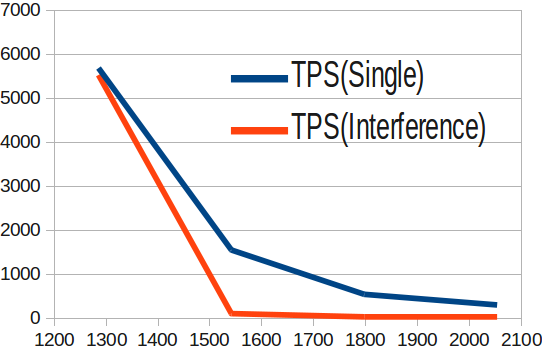
\includegraphics[width=4in]{images/MedScale.png}
  \caption{TPS with and without interference.  Moving from a Medium DB to a Large DB.}
  \label{fig:smallIO}
  \end{center}
\end{figure}

\subsubsection{Existing tools analysis}
\indent Trying to analyze the performance drop in Dom1 without knowing about this external interference is difficult.  
There were no changes to Dom1 when run by itself and run with other guests.  
By using the system \emph{sar} utility we can examine available memory, SwapIn and BytesIn/s to see if we can determine why the application benchmark is degraded without collecting external information (Figure \ref{fig:vmstat}).  
Memory is not used as efficiently, the system almost completely elimiates swapping data in, and also can't read as quickly from disk.  
However, there is no indication that the problem was due to an external guest and hypervisor using those resources.
A DBA looking at these numbers may conclude that kernel swap or DB tuning may fix the problem.  
The root cause of the performance drop is due to external interference, which is not known from examining the data available.

\begin{table}[h]
  \begin{tabular}{ l | r | r | r }
    VMstat & Single & Multiple & Drop \\ \hline
	Memory & 211Kb & 138Kb & 35\% \\
	SwapIn/s & 1,480 & 85 & 94\% \\
	BytesIn/s & 6,877 & 4,438 & 35\% \\
  \end{tabular}
\caption{Some resource statistics collected with vmstat on Dom1 on a Large database while running alone and with multiple systems.} 
\label{fig:vmstat}
\end{table}

% Section 7.2
\subsection{Personal Server}
In the previous experiment we showed the interference that can occur when exteranl I/O interference is applied to a guest domain.
In this experiment, we verify our design to show interference from external systems, when the system is I/O bound.
The results are from our IBM x3650, where each guest is configured to use 512MB of vRAM.
First, we run the benchmark with a 640MB database without interference and calcuate the overhead using the method in section 5.4.  
Then we start Dom2 - Dom4, run the benchmark in Dom1, and calculate the interference using the method in section 5.5.  
We compare the results of the calculated interference with the performance drop in the application.

\begin{Verbatim}
# xm list
Name                            ID   Mem VCPUs      State   Time(s)
Domain-0                        0  1988     4     r-----  88871.2
Test_VM1                        1   512     1     -b----  60187.0
Test_VM2                        2   512     1     -b----   5722.0
Test_VM3                        3   512     1     -b----   5273.0
Test_VM4                        4   512     1     -b----   5203.5
\end{Verbatim}

% Section 7.2.1
\subsubsection{Overhead}
We calculate the overhead for the guest OS paging and the I/O reads using the resource counters defined in our test suite.  While calculating the overhead we also collected the application performance at 415 TPS without any external interfernece.

% See Test7_1Results.xls (Barbaro - Exp7.2(P2))
\begin{table}[h]
\begin{tabular}{ l l l p{5cm} }
  Counter & Dom0 & Dom1 & $Overhead_V$ \\
  \hline
	pgpgin    & 332,504 & 165,901 & 100\% \\
	pgfault   &  25,648 & 132,691 & -81\% \\
	r sectors & 332,504 & 331,803 &   0\% \\
	r\_ms     &  63,356 &  72,428 & -13\% \\
	r total   &  11,145 &  12,166 &  -8\% \\
  \hline
\end{tabular}
\caption{I/O Overhead calculated average of four test runs on the IBM x3650.}
\label{tab:OverheadSmall}
\end{table}

One thing to notice is that the pgpgin from the Dom1 is about half of the host in Dom0, which results in 100\% overhead.  
We also see in Dom0 that pgpgin is exactly the same as the sectors read.  
After some research on this we believe that the Dom0 and guest kernels are reporting different units of measurements, and there is not really 2x overhead for the pgpgin statistic.  
In the Linux 2.4 and later kernel blocks and sectors were both 512 bytes, and the unit of measurement for pages in were reported in 1K sizes.  Since the Dom0 kernel is version 3.5.54 and the guest kernel is 2.6.32, we believe that the guest is reporting 1KB pages, and the Dom0 is reporting 512 byte pages to match the sector (and block) size. 

In order to report an accurate overhead, we would need to ensure that the unit of measurement for values reported between the guest and hypervisor are consistent.  For this report we will show the raw numbers, since the goal is to determine whether there is interference from an external layer. 

The other counters all show a negative overhead because the hypervisor performs less physical requests to disk and page faults than were completed in the guest.  For example the guest issued about 12 thousand reads, but the hypervior only actually executed 11 thousand total read requests.  This is likely due to optimizations in the hypervisor to cache data.

% Section 7.2.2
\subsubsection{Memory Interference}
We repeat the previous experiment with 4 guest domains all running at the same time.
Since the DB size in Dom1 is 640MB and there is 512MB of vRAM on Dom1, we can say that Dom1 is bound by disk I/O speed.
We run an experiments with the other 3 guest domains running a memory bound database.  Dom2 - Dom4 still has 512MB vRAM.  
We create a Small DB of 128MB in each of the other domains to generate memory interference on Dom1.
By using Equation 2 and 3 we can calculate the $Overhead_Vall$ and the $Interference$ for each counter.

\begin{table}[h]
\begin{tabular}{ l l l l p{5cm} }
  Counter & Dom0 & $\sum{DomU}$ & $Overhead_Vall$ & $Interference$ \\
  \hline
	pgpgin    & 328,144 & 163,784 & 100\% &   0\% \\
	pgfault   &  57,293 & 481,541 & -88\% &  -7\% \\
	r sectors & 328,144 & 256,352 &  28\% &  28\% \\
	r ms      & 103,483 &  70,751 &  46\% &  59\% \\
	r total   &  13,365 &   9,547 &  40\% &  48\% \\
  \hline
\end{tabular}
\caption{Interference calculated from Small 128MB DB in Dom2 - Dom4.  TPS dropped by 20\%} 
\label{fig:InterferenceSm}
\end{table}

From these tests, Dom1 had 331 TPS, and was degraded from 415 TPS.  We see significant interference in the read counters.  It is not shown in these results, but Dom2 - Dom4 was able to cache the entire working set in memory and did not issue any read requests.  Dom1 was the only domain to issue read request. The totals from all guests domains for each of the three read counters is exactly the same as Dom1.  We can see that the hypervisor read statistics were significantly greater than when we calcualted the overhead.  We also notice that there are less page faults in the hypervisor than there was when collecting overhead.

% Section 7.2.3
\subsubsection{I/O Interference}
Now we create I/O Interference in the three guest domains by creating a 640MB Large DB in Dom2 - Dom4.  Since each guest has 512MB vRAM, this should cause significant I/O contention in Dom1.

\begin{table}[h]
\begin{tabular}{ l l l l p{5cm} }
  Counter & Dom0 & $\sum{DomU}$ & $Overhead_Vall$ & $Interference$ \\
  \hline
	pgpgin    & 549,419 & 274,533 & 100\% &   0\% \\
	pgfault   &  58,201 & 255,232 & -77\% &   3\% \\
	r sectors & 549,419 & 378,075 &  46\% &  46\% \\
	r ms      & 285,334 & 184,588 &  55\% &  67\% \\
	r total   &  20,723 &  14,169 &  47\% &  55\% \\
  \hline
\end{tabular}
\caption{Interference calculated Large 640MB DB in Dom2 - Dom4.  TPS dropped by 39\%}
\label{fig:InterferenceLg}
\end{table}

During these tests, the application benchmark Dom1 showed 254 TPS.  This is much less than when run without interference (415 TPS) and with memory interference (331TPS).  All of the read counters showed significant interference.  Additionally we are showing some interference from page faults.  The overhead is still negative for all of the page faults compared to the page faults in Dom0.  But it is less than it was when originally collecting the overhead.

\subsection{Business Server}
For this experiment we use our Dell server with 12GB of physical RAM. We configure all Dom1 to use 2GB of vRAM and keep Dom2 - Dom4 at 1GB of vRAM. We create an I/O bound application by creating a 3 GB database in each domain. For this size of database expect to see a significant change in the application
when the external guest domains (Dom2 - Dom4) compete for physical resources with Dom1.

\subsubsection{Use partial memory}
\begin{Verbatim}
Name                 ID   Mem VCPUs      State   Time(s)
Domain-0              0  2048    16     r-----  22461.6
TestVM1               1  2048     1     -b----   1100.6
TestVM2               2  1024     2     -b----   1095.0
TestVM3               3  1024     1     -b----   1037.5
TestVM4               4  1024     2     -b----   1170.8
\end{Verbatim}

We calculate the $Overhead$ and $Interference$ in Dom1 using the same method as described previously. 
According to these results (Table \ref{tab:IntMedA}) this did not generate the same type of performance problems as when run in the previous example.  
There was a significant drop in the application TPS, but these performance counters did not show why there was a significant application performance degradation (327 TPS - 71 TPS).

\begin{table}[h]
\begin{tabular}{ l r r r r r p{5cm} }
	         & pgpgin & pgfault & r sectors & r ms	& r total & TPS \\
	\hline
	$Overhead_V$ & 100\%  & -61\%	 &      0\%	 & -10\% &    -8\% &  327 \\
\end{tabular}
\caption{Average Overhead in Dom1 with 2GB vRAM}
\end{table}

\begin{table}[h]
\begin{tabular}{ l r r r r r p{5cm} }
	Domain  & pgpgin & pgfault & r sectors & r ms	& r total & TPS \\
	\hline
	Dom-0	& 174560 &	55192 &	174560 &	325579 &	5560 & N/A \\
    Dom-U	& 87280	 & 213934 & 174560 &    374942 &    5951 & N/A \\
	$Overhead_Vall$ & 100\%  &   -74\%&  0\%   &    -13\% &    -6\%  & N/A \\
    $Interference$ & 0\% & -13\% & 0\%   &     -3\% &     1\%  & 71 \\
\end{tabular}
\caption{Interference with 4 guest domains running concurrently.}
\label{tab:IntMedA}
\end{table}

We calculated the reads per second at each layer (Table \ref{fig:rps}) during the calculation of the overhead and the calculation of the Interference by using the total reads divided by the time spent reading.    We can see a performance drop in in $Read/S$, but they are nearly identical between the guests and the hypervisor.  
\begin{table}[!h]
\begin{tabular}{ l r r p{5cm} }
	Experiment     & Dom0 & DomU  & TPS(Dom1) \\
	\hline
    Dom1 (Only)    & 67 & 65 & 327 \\
    Dom1 + 1 guest & 32 & 33 & 152 \\
    Dom1 + 3 guests& 16 & 17 &  71 \\
\end{tabular}
\caption{Reads/second from the view of the hypervisor and guests}
\label{fig:rps}
\end{table}

From this we can see that the hypervisor is degraded, and the application does not read as quickly.  There is interference caused by the external guest machines, but it does not appear to be from the same type of problems as in the previous experiment. The information obtained here is not enough to distinguish between a slow running guest application and external interference.

\subsubsection{Use all memory}
We re-configure all Dom1 to use 4GB of vRAM and increase the memory in Dom2, Dom3, and Dom4. We want to see if the extra memory in Dom0 is being used better and not showing the interference.
We create a medium size database in Dom1 of 3.2GB, which is slighly less than the available memory in Dom1. 

\begin{Verbatim}
Name                            ID   Mem VCPUs      State   Time(s)
Domain-0                         0   872    16     r-----  27116.4
TestVM1                          1  4096     1     -b----   1127.7
TestVM2                          2  3072     2     -b----   1735.8
TestVM3                          3  2048     1     -b----   1588.1
TestVM4                          4  2048     2     -b----   1906.1
\end{Verbatim}

We re-calculate the $Overhead$ for this configuration even though the results are similar to the previous two experiments.

\begin{table}[h]
\begin{tabular}{ l r r r r p{5cm} }
    Domain &  pgpgin &   pgfault & r\_sectors & r\_ms & r\_total \\
    \hline
    Dom-0  &  230512 &   23565   & 230512   & 108168 &  7990 \\
    Dom-1  &  115256 &   81480   & 230512   & 114090 &  8213 \\
$Overhead_V$ & 100\% &   -71.9\% & 0.0\	    & -4.5\%  & -2.2\% \\
    \hline
\end{tabular}
\caption{Overhead for VM and I/O statistics in 4GB Dom1.}
\label{fig:OverheadMed}
\end{table}

In the previous experiment we started 4 guest machines at the same time.  Now we calculate the interference with 2, 3, and 4 machines.   This allows us to compare how accurate the method is for calculating the interference.  As more guest machines are added, more interfernce should be observed in the guest. 

\begin{table}[h]
\begin{tabular}{ l r r r r r p{5cm} }
    Domains &  TPS & pgpgin &   pgfault & r\_sectors & r\_ms & r\_total \\
    \hline
    1 only & 1,348 & 0.0\%  &    0.0\%  &  0.0\%     &  0.0\% &   0.0\%  \\
    1 - 2  &  703  & -1.3\% &	-7.6\%  &  0.6\%     &  -3.5\% &  -3.2\%  \\
    1 - 3  &  543  & -2.3\% & 	-5.0\%  &  1.2\%     &  -6.1\% &  -7.7\%  \\
    1 - 4  &  277  & -3.2\% &   -5.9\%  &  1.6\%     & -11.1\% &  -12.7\% \\
    \hline
\end{tabular}
\caption{TPS in Dom1 and calculated interference for several counters.}
\label{fig:InterferenceMed}
\end{table}

We are still seeing a negative interference (Table \ref{fig:InterferenceMed}).  Furthermore there is less interference calculated as more external domains are added.  
It was stated earlier the a negative overhead (or interference) is actually the hypervisor doing less work.  
Our tests confirm that the hypervisor is sending less physical requests to disk than are being sent from all guests.  
However, the I/O throughput (reads/s) are degraded equally at both the hypervisor and the guest layers.  

We could argue that this could be a method to view the interference.  
We tried to prove this but found that there could be other reasons for these types of improvements which are not a result of external interference.  
So this type of negative interference can't be used to show interference from external systems. 
There must be an explanation for this degradation in the application, which is undetectable with our current method.

% Section 7.4
\subsection{Addtional counters}
We need to go back to our original assumption that we need to evaluate at ALL layers of the stack.  We also need to examine other counters to see if there is some indication of the problem.  In the Linux 2.6 kernel CPU wait time was added as a way to track time the CPU was idle, due to an I/O operation.  Instead of using the $/proc$ filesystem to read the counters and pass them, we just run the \emph{vmstat} command in the guest domain Dom1.  We do this while running without interference, and while running with two, three, and four guests simultaneously.

\subsubsection{I/O Wait Time}
According to the CPU Wait time from vmstat (Table \ref{tab:vmstat}), the guest domain is "Waiting on I/O".  
But there is no indication without additional information that the guest is waiting because additional guests are using the device.

\begin{table}[h]
\begin{tabular}{ l p{5cm} }
    Guests &  CPU Wait \\
    \hline
    1 only &  33  \\
    1 - 2  &  69  \\
    1 - 3  &  78  \\ 
    1 - 4  &  98  \\
    \hline
\end{tabular}
\caption{CPU wait time from a 5 second sample using vmstat in Dom1.}
\label{tab:vmstat}
\end{table}

\subsubsection{Additional Interference}
According to the Citrix XenServer manual, there is an additional layer we are missing from our data.   
The DomU guests all write to a parvirtualized disk driver in /dev/xvda.  Which is managed by a kernel module in the guest machine (blkfront).  This driver then passes data to a kernel driver in Dom0 (blkback).  The blkback driver then communicates with a blacktap driver driver which will read/write from/to the Virual Device Infrastructure.   When the two drivers communicate they track disk I/O statistics similar to the /proc/diskstat that we used previously.  For Xen the communication between the two drivers is done as a block device.  One block device for each guest domain.

We use the \emph{IOstat} command to read statistics from this block device.  The IOstat command works by reading kernel counters and aggregating results similar to our method.  We examime 4 counters from a 5 second sample when the guest domain is running with and without interference.  We compare these results to the physical block device in Dom0.
Further research on these fields explain that these are aggregated results of statistics from \emph{/proc/diskstats}, but from fields we did not collect during our experiments.


\begin{description}
	\item{avgqu-sz} The average queue length of the requests that were issued to the device.
	\item{await} The average  time  (in  milliseconds)  for  I/O  requests issued to the device to be served. This includes the time spent by the requests in queue and the time spent servic‐ ing them.
	\item{svctm} The  average  service  time  (in  milliseconds)  for  I/O requests that were issued to the device. 
	\item{\%util} Percentage of CPU time during  which  I/O  requests  were issued  to  the  device  (bandwidth  utilization  for the device). Device saturation  occurs  when  this  value  is close to 100\%.
\end{description}

\begin{table}[htbp]
\begin{tabular}{|l|l|r|r|r|r|}
\hline
 & Device: & \multicolumn{1}{l|}{avgqu-sz} & \multicolumn{1}{l|}{await} & \multicolumn{1}{l|}{svctm} & \multicolumn{1}{l|}{\%util} \\ \hline
Physical & sda & 3.54 & 12.23 & 2.85 & 82.52 \\ \hline
Dom1 & tda & 3.67 & 12.51 & 2.79 & 81.8 \\ \hline
\textbf{Overhead} & \textbf{} & \textbf{-4\%} & \textbf{-2\%} & \textbf{2\%} & \textbf{1\%} \\ \hline
\end{tabular}
\caption{One Guest}
\label{1guest}
\end{table}

\begin{table}[htbp]
\begin{tabular}{|l|l|r|r|r|r|}
\hline
 & Device: & \multicolumn{1}{l|}{avgqu-sz} & \multicolumn{1}{l|}{await} & \multicolumn{1}{l|}{svctm} & \multicolumn{1}{l|}{\%util} \\ \hline
Physical & sda & 8.38 & 36.05 & 4.27 & 100 \\ \hline
Dom1 & tda & 5.25 & 42.44 & 7.27 & 92.22 \\ \hline
Dom2 & tdb & 3.4 & 28.78 & 8.53 & 100 \\ \hline
Avg/Sum &  & 8.65 & 35.61 & 7.9 & 96.11 \\ \hline
Overhead &  & 3\% & -1\% & 46\% & -4\% \\ \hline
Interference &  & 7\% & 1\% & 44\% & -5\% \\ \hline
\end{tabular}
\caption{Two guests}
\label{2guest}
\end{table}

\begin{table}[htbp]
\begin{tabular}{|l|l|r|r|r|r|}
\hline
 & Device: & \multicolumn{1}{l|}{avgqu-sz} & \multicolumn{1}{l|}{await} & \multicolumn{1}{l|}{svctm} & \multicolumn{1}{l|}{\%util} \\ \hline
Physical & sda & 10.36 & 48.15 & 4.98 & 100 \\ \hline
Dom1 & tda & 4.47 & 56.48 & 12.31 & 94.76 \\ \hline
Dom2 & tdb & 3.59 & 36.66 & 10.16 & 100 \\ \hline
Dom3 & tdc & 2.02 & 58.81 & 29.06 & 99.98 \\ \hline
Avg/Sum &  & 10.08 & 50.65 & 17.18 & 98.25 \\ \hline
Overhead &  & -3\% & 5\% & 71\% & -2\% \\ \hline
Interference &  & 1\% & 7\% & 69\% & -3\% \\ \hline
\end{tabular}
\caption{Three guests}
\label{3guest}
\end{table}

\begin{table}[htbp]
\begin{tabular}{|l|l|r|r|r|r|}
\hline
Physical & Device: & \multicolumn{1}{l|}{avgqu-sz} & \multicolumn{1}{l|}{await} & \multicolumn{1}{l|}{svctm} & \multicolumn{1}{l|}{\%util} \\ \hline
Physical & sda & 9.83 & 60.87 & 6.94 & 100 \\ \hline
Dom1 & tda & 2.81 & 139.5 & 40.24 & 99 \\ \hline
Dom2 & tdb & 2.31 & 210.11 & 69.44 & 100 \\ \hline
Dom3 & tdc & 2.11 & 39.25 & 18.59 & 100 \\ \hline
Dom4 & tdd & 2.13 & 39.52 & 18.59 & 100 \\ \hline
Avg/Sum &  & 9.36 & 107.10 & 36.72 & 99.75 \\ \hline
Overhead &  & -5\% & 43\% & 81\% & 0\% \\ \hline
Interference &  & -1\% & 45\% & 79\% & -1\% \\ \hline
\end{tabular}
\caption{Four guests}
\label{4guest}
\end{table}

By looking at this additional layer of information we can determine where the interference is occuring.  In this case we are essentially using additional fields in /proc/diskstats which we did not collect in the original sets of tests.  We can calculate the svctm and await time using CPU and diskstat statistics at all layers of virtualization.

\subsubsection{How to calculate}
The utilization (\emph{\%util}) is the time spent in the I/O (CPU Wait Time) divided by the sample period.  The Linux kernel tracks the CPU wait time in 2.6 and later kernels.  Since our method controls the frequecy at which to calculate this information we can track the sample and calcualte the utilization.

The service time (\emph{svctime}) is the utilization percentage divided by the throghput.  The throughput is the number of I/O operations per second (IOPS).  When the utilization is near 100\%, this is just the inverse of the throughput. This is supposed to represent the time when a request leaves the queue until it has completed processing.  However, the man page warns that this is not an accurate measurement of the actual service time.

The average wait time (\emph{await}) is the time the I/O request was in queue and the time it took to process the request.  One of the counters in /proc/diskstat shows the "weighted" time in milliseconds \cite{iostats}.  

\begin{Verbatim}
Field  9 -- # of I/Os currently in progress
    The only field that should go to zero. Incremented as requests are
    given to appropriate struct request_queue and decremented as they finish.
Field 10 -- # of milliseconds spent doing I/Os
    This field increases so long as field 9 is nonzero.
Field 11 -- weighted # of milliseconds spent doing I/Os
    This field is incremented at each I/O start, I/O completion, I/O
    merge, or read of these stats by the number of I/Os in progress
    (field 9) times the number of milliseconds spent doing I/O since the
    last update of this field.  This can provide an easy measure of both
    I/O completion time and the backlog that may be accumulating.
\end{Verbatim}

We did not include these in our original tests becuse Field 9 was always zero.  This was due to the fact that our sample was taken before and after the test load was created.  It would have been better to get the queue length and wait time at all layers and at more frequent samples during the test load.


% Section 7.5
\subsection{Verification without interference}
In the previous two experiments, we showed how our method can give a guest domain vital information when it is degraded from external interference.  However, what if the guest domain was degraded due to an application bug, DB change, or misconfiguration?   In that case we want our method to show that there is not any external interference.

We have previously demonstrated that the database TPS can become degraded as the size of the database increases.  Now we show that by simply increasing the I/O load from a single domain, that our method does not report external interfernce.In this case the application is degraded because the working set exceeds the available memory.  The application depends on the I/O system for performance, but it is not degraded from external interference.

We begin by using Table \ref{1guest} as the value for the $Overhead$, and then increase the DB size in Dom1 and calculate the external $Interference$ as well as the TPS when the DB increases.  Our Dom1 has 4GB of vRAM available.



